\chapter{MS-RPC: Microsoft Remote Procedure Call}


\section{links}
\begin{itemize}
    \item
        \href{https://learn.microsoft.com/en-us/windows/win32/rpc/rpc-start-page}{Remote procedure call (RPC)}
    \item
        \href{https://www.akamai.com/fr/blog/security-research/msrpc-security-mechanisms}{Présentation du MS-RPC et de ses mécanismes de sécurité}
    \item
        \href{https://juggernaut-sec.com/ad-recon-msrpc/}{AD Recon – MSRPC}
    \item
        \href{https://clearbluejar.github.io/posts/surveying-windows-rpc-discovery-tools/}{A Survey of Windows RPC Discovery Tools}
    \item 
        \url{https://book.hacktricks.xyz/network-services-pentesting/135-pentesting-msrpc}
    \item
        \url{https://0xffsec.com/handbook/services/msrpc/}

\end{itemize}


\section{Introduction}

\subsection{Description}
\href{https://en.wikipedia.org/wiki/Microsoft_RPC}{MSRPC (Microsoft Remote
Procedure Call)} is a protocol commonly related to SMB.  RPC provides an
application developer a generic way to execute a procedure in a local or remote
process without having to understand the network protocols used to support the
communication, as specified in
\href{https://docs.microsoft.com/en-us/openspecs/windows_protocols/ms-rpce/290c38b1-92fe-4229-91e6-4fc376610c15}{MS-RPCE},
which defines an RPC over SMB Protocol that can use SMB Protocol named pipes as
its underlying transport.


Depending on the host configuration, the RPC endpoint mapper can be accessed:
\begin{itemize}
    \item through TCP and UDP port 135
    \item via SMB with a null or authenticated session (TCP
139 and 445)
    \item  as a web service listening on TCP port 593.
    \item via a local SMB pipe
\end{itemize}


The MSRPC process begins on the client side, with the client application
calling a local stub procedure instead of code implementing the procedure. The
client stub code retrieves the required parameters from the client address
space and delivers them to the client runtime library, which then translates
the parameters into a standard Network Data Representation format to transmit
to the server.

The client stub then calls functions in the RPC client runtime library to send
the request and parameters to the server. If the server is located remotely,
the runtime library specifies an appropriate transport protocol and engine and
passes the RPC to the network stack for transport to the server.

The client stub then calls functions in the RPC client runtime library to send
the request and parameters to the server. If the server is located remotely,
the runtime library specifies an appropriate transport protocol and engine and
passes the RPC to the network stack for transport to the server. For more
details, please check
\href{https://blog.openthreatresearch.com/ntobjectmanager_rpc_smb_scm}{this
link}.

\begin{figure}
  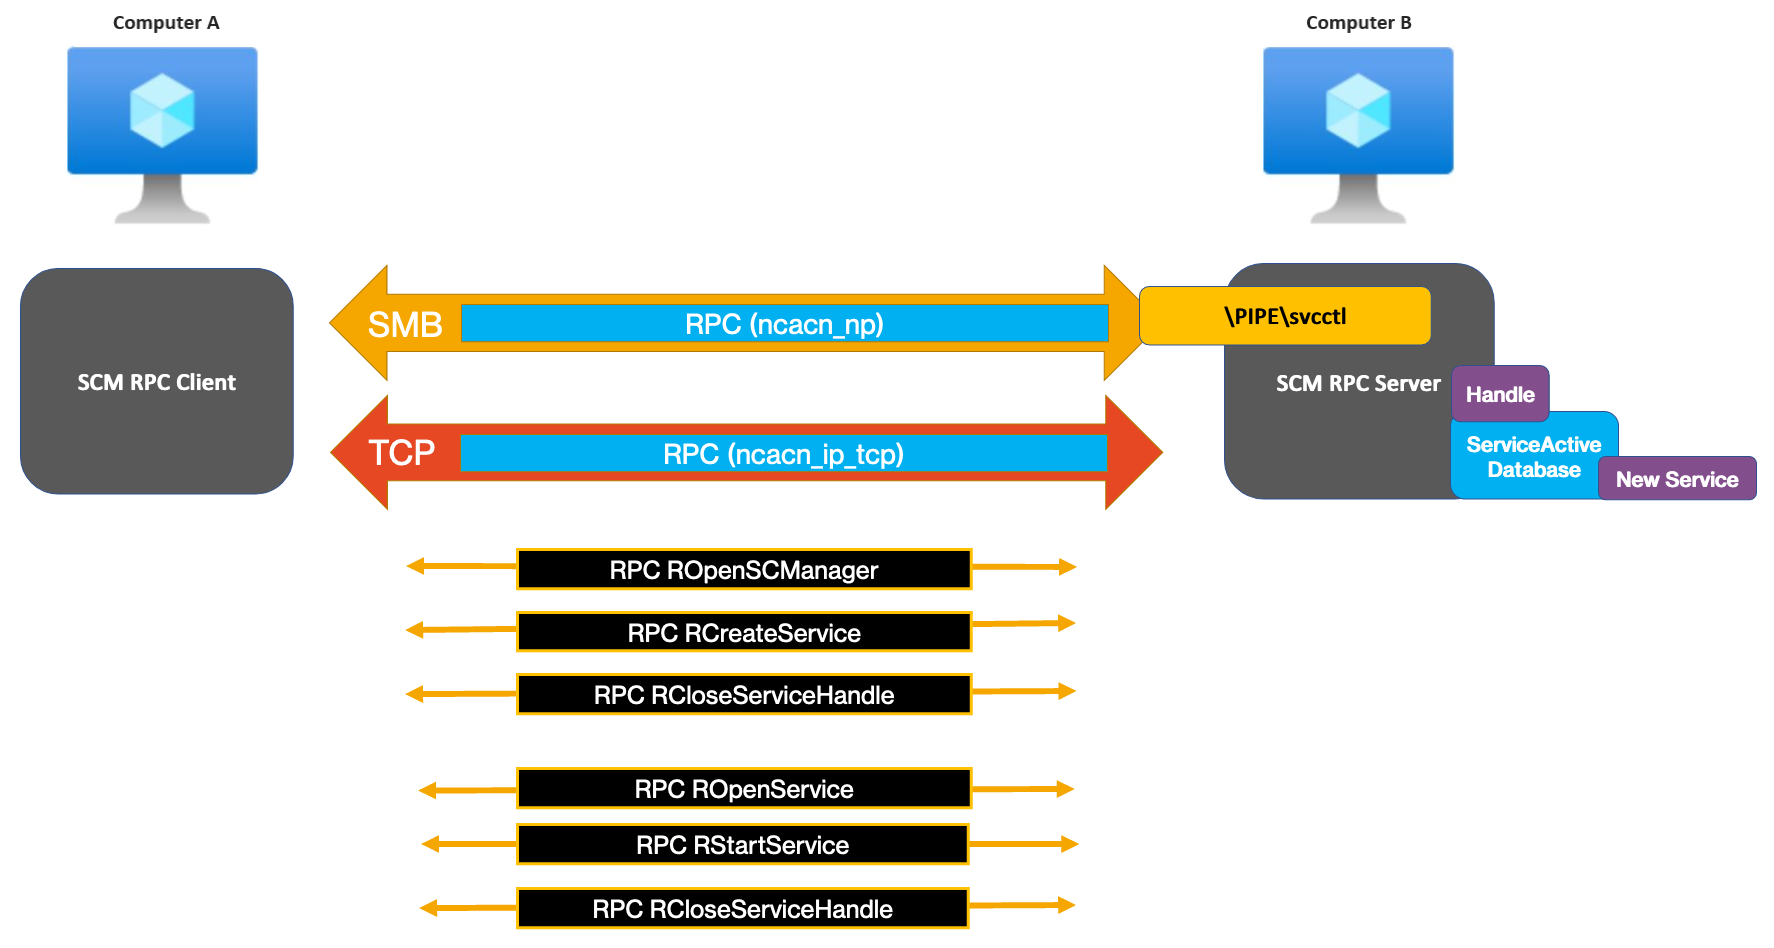
\includegraphics[width=\linewidth]{network/msrpc/images/msrpc.png}
  \caption{MSRPC protocol}
  \label{fig:msrpc}
\end{figure}


Un service RPC Windows peut etre accessible via differents protocoles de
transport, les plus frequents etant :
\begin{itemize}
\item un pipe utilise par le protocole reseau Windows SMB/CIFS (\verb+ncacn_np+) ;
\item le protocole reseau TCP (\verb+ncacn_ip_tcp+) ;
\item le protocole reseau UDP (\verb+ncacn_ip_udp+) ;
\item le protocole HTTP (\verb+ncacn_http+) ;
\item un pipe SMB/CIFS local (\verb+ncalrpc+).
\end{itemize}
Lorsque le protocole de transport utilise est SMB/CIFS le service RPC est
en ecoute sur les ports TCP 139 et 445. S’il s’agit de TCP ou UDP le port doit
etre precise lors de la creation du service. Un client peut connaıtre le port en
interrogeant le service \verb+portmapper+ en ecoute sur le port TCP 135.
L’ensemble des protocoles de transport utilises par un service RPC est defini
au sein d’un point final (\verb+endpoint+ et a le format suivant :
\begin{verbatim}
endpoint("ncacn_ip_tcp:[2046]", "ncacn_np:[\\pipe\\rpc_service]");
\end{verbatim}

L’exemple precedent represente un service RPC en ecoute sur le port TCP
2046 et egalement disponible via le protocole reseau SMB/CIFS.

Un service RPC contient enfin une ou plusieurs interfaces servant a decrire
toutes les fonctions utilisees ainsi que tous les points finaux disponibles. Une
interface RPC est representee par un identifiant (
\verb+uuid (00000001-0002-0003-0004-000000000005)+), un numero de version
(\verb+version (1.0)+), des points finaux (optionnels). Le lecteur est invite a
lire
\href{https://papers.vx-underground.org/papers/Windows/Network%20Communications/Windows%20Network%20Services%20Internals.pdf}{Windows
network services internals} pour une liste complete des services RPC Windows.

L’ensemble des caracteristiques permettant de d ecrire un service MSRPC
sont contenues dans un fichier texte (\verb+service.idl+) utilisant le langage MIDL.


\subsection{Security}
 MSRPC interfaces can be abused by attackers to collect valuable information or
 compromise servers. Many Windows administration tools, such as \verb+PsExec+ and
 PowerShell, depend on MSRPC. Attackers can perform Active Directory
 reconnaissance (to identify domain administrator accounts on the network) by
 directly requesting information from Windows workstations or domain
 controllers with MSRPC. An attacker with elevated privileges and access to
 these tools can leverage MSRPC to send malicious commands to remote servers.
 After compromising those servers, the attacker can pivot, or laterally move,
 to new targets on the network.

\subsection{Notable RPC interfaces}
RPC services over an SMB transport, i.e. port 445/TCP, are reachable through
\verb+named pipes+ (through the \verb+IPC$+ share). There are many interesting
named pipes that allow various operations from \verb+NULL+ sessions context, to
local administrative context.

\begin{itemize}
    \item \verb+\pipe\lsarpc+: enumerate privileges, trust relationships, SIDs,
        policies and more through the LSA (Local Security Authority)
    \item \verb+\pipe\samr+: LSA SAMR interface, used to access public SAM
        database elements (e.g., usernames) and brute-force user passwords
        regardless of account lockout policy Oreilly library enumerate domain
        users, groups and more through the local SAM database (only works pre
        Win 10 Anniversary)
    \item \verb+\pipe\atsvc+: Task scheduler, used to remotely execute commands
        used by impacket \verb+atexec+~\ref{tool:impacket:atexec}
    \item \verb+\pipe\winreg+: Remote registry service, used to access the system registry
    \item \verb+\pipe\svcctl+: Service control manager and server services,
        used to remotely start and stop services and execute commands used by
        impact \verb+psexec+~\ref{tool:impacket:psexec} and
        \verb+smbexec+~\ref{tool:impacket:smbexec}
    \item \verb+\pipe\srvsvc+: Service control manager and server services, used to remotely start and stop services and execute commands
    \item \verb+\pipe\epmapper+: used by DCOM (Distributed Component Object
        Model), itself used by WMI (Windows Management Instrumentation), itself
        abused by attackers for command execution (used by Impacket
        \verb+wmiexec+~\ref{tool:impacket:wmiexec}) COM is also used by MMC
        (Microsoft Management Console), itslef abused by attackers for command
        execution (Impacket's \verb+dcomexec+~\ref{tool:impacket:dcomexec})
\end{itemize}

\subsection{Null sessions}
NULL sessions are unauthenticated SMB sessions that allow attackers to operate
RPC calls through SMB named pipes without being authenticated first. This
allows for many recon techniques like the enumeration of domain and local
information (users, groups, RIDs, SIDs, policies, etc.).

\subsection{Recon through interesting named pipes}

\section{Fingerprinting}

\subsection{nmap}
\begin{verbatim}
nmap -sV -p135 10.10.x.x
nmap -p135 --script=msrpc-enum 10.10.x.x
\end{verbatim}


\section{Enumeration}
\subsection{Identifying Exposed RPC Services}
You can query the RPC locator service and individual RPC endpoints to catalog
interesting services running over TCP, UDP, HTTP, and SMB (via named pipes).
Each IFID value gathered through this process denotes an RPC service (e.g.,
5a7b91f8-ff00-11d0-a9b2-00c04fb6e6fc is the Messenger interface).

Todd Sabin’s rpcdump and ifids Windows utilities query both the RPC locator and
specific RPC endpoints to list IFID values. The rpcdump syntax is as follows:
\begin{verbatim}
rpcdump [-p port] 192.168.189.1
\end{verbatim}

\begin{verbatim}
use auxiliary/scanner/dcerpc/endpoint_mapper
use auxiliary/scanner/dcerpc/hidden
use auxiliary/scanner/dcerpc/management
use auxiliary/scanner/dcerpc/tcp_dcerpc_auditor
rpcdump.py <IP> -p 135
\end{verbatim}

\subsection{RID Cycling}

RID Cycling is a method that allows attackers to enumerate domain objects by
bruteforcing or guessing RIDs and SIDs, based on the fact that RIDs are
sequential.

\href{https://github.com/trustedsec/ridenum}{ridenum} an be used to operate
that recon technique, with a Null session or with an authenticated one.

\verb+crackmapexec+~\ref{tool:crackmapexec} can also be used with
\verb+--rid-brute+

\subsection{rpcclient}
\verb+rpcclient+~\ref{tool:rpcclient} an be used to operate recon through MS-RPC
services behind SMB named pipes. It offers multiple useful commands.






